% ===========================================================================
% Mesurer la similarité
% Traduit et adapté de :
%   https://www.bootstrapworld.org/materials/fall2026/en-us/lessons/measuring-similarity/
% Licence : Creative Commons 4.0 Unported (Bootstrap Community)
% ===========================================================================

\documentclass[12pt,a4paper]{article}

% ---------- Packages ----------
\usepackage[utf8]{inputenc}
\usepackage[T1]{fontenc}
\usepackage{libertine}
\usepackage{microtype}
\usepackage[french]{babel}
\usepackage{graphicx}
\usepackage{float}
\usepackage{hyperref}
\usepackage{geometry}
\usepackage{enumitem}
\usepackage{tabularx}
\usepackage{xcolor}
\usepackage{colortbl}
\usepackage[raster]{tcolorbox}
\usepackage{booktabs}
\usepackage{fancyhdr}
\usepackage{titlesec}
\usepackage{amsmath}
\usepackage{amssymb}
\usepackage{listings}

% ---------- Mise en page ----------
\geometry{margin=2.5cm, headheight=15pt, footskip=30pt}
\fancyhf{}
\fancyhead[L]{\textbf{Mesurer la similarité}}
\fancyhead[R]{\thepage}
\fancyfoot[C]{Bootstrap Community — CC BY 4.0}
\renewcommand{\headrulewidth}{0.4pt}
\pagestyle{fancy}

% ---------- Couleurs ----------
\definecolor{bsblue}{RGB}{41,128,185}
\definecolor{bsgreen}{RGB}{39,174,96}
\definecolor{bsorange}{RGB}{230,126,34}
\definecolor{bsgray}{RGB}{149,165,166}
\definecolor{codebg}{RGB}{245,247,250}

% ---------- Styles de sections ----------
\titleformat{\section}[hang]{\Huge\bfseries\color{bsblue}}{}{0pt}{}[\vspace{-0.5em}\rule{\textwidth}{2pt}]
\titleformat{\subsection}[hang]{\Large\bfseries\color{bsblue!80!black}}{}{0pt}{}
\titleformat{\subsubsection}[hang]{\large\bfseries\color{bsgreen!60!black}}{}{0pt}{}

% ---------- Environnements personnalisés ----------
\newtcolorbox{overviewbox}{
  colback=bsblue!5!white, colframe=bsblue!60!white,
  fonttitle=\bfseries, title=Objectif de la section,
  left=1em, right=1em, top=0.5em, bottom=0.5em
}
\newtcolorbox{activitybox}{
  colback=bsgreen!5!white, colframe=bsgreen!60!white,
  fonttitle=\bfseries, title=Activité,
  left=1em, right=1em, top=0.5em, bottom=0.5em
}
\newtcolorbox{thinkbox}{
  colback=bsorange!5!white, colframe=bsorange!60!white,
  fonttitle=\bfseries, title=Réflexion,
  left=1em, right=1em, top=0.5em, bottom=0.5em
}
\newtcolorbox{keypointbox}{
  colback=bsgray!10!white, colframe=bsgray!50!white,
  fonttitle=\bfseries, title=Point clé,
  left=1em, right=1em, top=0.5em, bottom=0.5em
}
\newtcolorbox{instructornotes}{
  colback=yellow!10!white, colframe=yellow!80!black,
  fonttitle=\bfseries, title=Notes pour l'enseignant·e,
  left=1em, right=1em, top=0.5em, bottom=0.5em
}
\newtcolorbox{codebox}{
  colback=codebg, colframe=bsgray!40,
  fonttitle=\bfseries, title=Code Pyret,
  left=1em, right=1em, top=0.5em, bottom=0.5em
}
\newtcolorbox{contractbox}{
  colback=bsblue!3!white, colframe=bsblue!40!white,
  left=1em, right=1em, top=0.6em, bottom=0.6em
}

% ---------- Style listings pour Pyret ----------
\lstdefinelanguage{Pyret}{
  keywords={use,context,url-file,and,or,not,if,else,for,fun,data,sharing,include,import,as,where,let,rec,is,=,true,false,end,Table,String,Number,Boolean,Image,Row,List,Code},
  sensitive=true,
  comment=[l]{\#},
  morestring=[b]",
  morestring=[b]',
}
\lstset{
  language=Pyret,
  basicstyle=\ttfamily\small,
  commentstyle=\color{bsgreen!70!black}\itshape,
  keywordstyle=\color{bsblue}\bfseries,
  stringstyle=\color{bsorange},
  backgroundcolor=\color{codebg},
  frame=single,
  framesep=5pt,
  rulecolor=\color{bsgray!40},
  breaklines=true,
  breakatwhitespace=false,
  showstringspaces=false,
  aboveskip=0.8em,
  belowskip=0.8em,
}

% ---------- Commandes pratiques ----------
\newcommand{\img}[3]{%
  \begin{figure}[H]
    \centering
    \includegraphics[#2]{#1}
    \caption{#3}
    \label{fig:#1}
  \end{figure}
}
\newcommand{\contrat}[1]{%
  \begin{contractbox}
    \ttfamily #1
  \end{contractbox}
}

% ---------- Informations du document ----------
\title{%
  \vspace{-2cm}
  {\Huge\bfseries Mesurer la similarité}\\[0.5em]
  {\large Représenter des documents comme des points dans l'espace~: sacs de mots, distance et angle}\\[1em]
  {\normalsize Traduit et adapté depuis \href{https://www.bootstrapworld.org/materials/fall2026/en-us/lessons/measuring-similarity/}{Bootstrap World} (Fall 2026)}\\[0.5em]
  {\normalsize Licence Creative Commons 4.0 International}
}
\date{}
\author{}

\begin{document}

\maketitle
\thispagestyle{empty}

\vspace{2cm}
\begin{center}
  \textit{Ces supports ont été développés en partie grâce au soutien de la National Science Foundation\\
  (bourses 1042210, 1535276, 1648684, 1738598, 2031479 et 1501927).}
\end{center}

\newpage
\tableofcontents
\newpage

% ===========================================================================
% SECTION 1 : COMMENT LES ORDINATEURS « VOIENT »-ILS ?
% ===========================================================================
\section{Comment les ordinateurs «~voient~»-ils~?}

\begin{overviewbox}
  Les élèves explorent les façons dont les attributs des images peuvent être calculés, en utilisant diverses fonctions.
\end{overviewbox}

% ---------- Launch ----------
\subsection{Lancement}

Dans \href{https://images.google.com/}{Google Image Search}, vous pouvez faire glisser une image dans la barre de recherche et demander à Google de trouver d'autres images \emph{similaires}. La recherche d'images est essentiellement un \textbf{système de recommandation}, où l'utilisateur·trice téléverse une image qu'iel aime et Google produit une liste de correspondances recommandées.

\begin{center}
  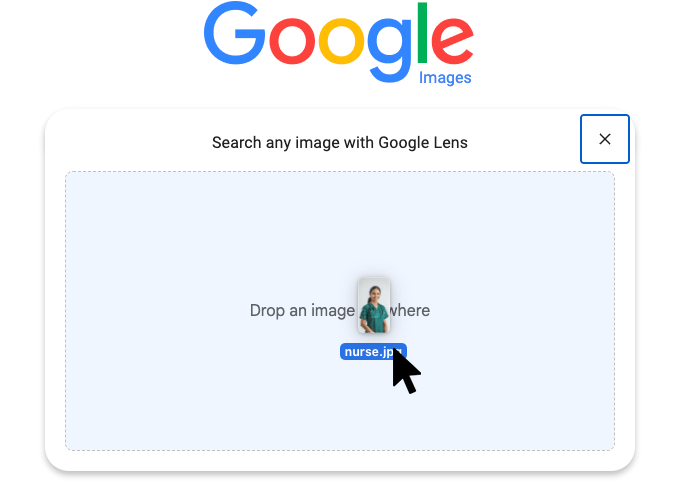
\includegraphics[width=0.45\textwidth]{images/df1a0a6dcdab181c.png}\hfill
  
\includegraphics[width=0.45\textwidth]{images/039d24b09872b565.png}
\end{center}
\begin{center}
\small\emph{Gauche~: faire glisser une image dans la barre de recherche Google Images. Droite~: les premiers résultats d'une recherche d'images similaires.}
\end{center}

\begin{activitybox}
  \begin{itemize}
    \item Ouvrez le \textbf{fichier Images Similaires} (\texttt{Images\allowbreak-Similaires\allowbreak-Starter.arr}) sur votre ordinateur et enregistrez-en une copie qui n'appartient qu'à vous. Cliquez sur «~Run~».
    \item Il y a beaucoup de définitions dans ce fichier~! Expérimentez avec elles dans la Zone d'Interactions pour voir ce qu'elles font.
  \end{itemize}
\end{activitybox}

\img{images/9039e2d6a0203ce2.png}{width=0.7\textwidth}{Les 9~images de montagnes utilisées dans le fichier Pyret, étiquetées avec leurs numéros d'identification.}

\begin{activitybox}
  Évaluez \texttt{mountains} dans la \textbf{Zone d'Interactions}, puis cliquez sur la vignette pour l'agrandir.

  \begin{itemize}
    \item \textbf{Quels attributs ces neuf images partagent-elles~? Qu'est-ce qui les rend similaires~?}
    \item \textbf{Quels attributs distinguent ces neuf images~? Qu'est-ce qui les rend différentes~?}
    \item \textbf{Laquelle est la \emph{plus} similaire à \texttt{sun1}~: \texttt{day1} ou \texttt{day2}~? Pourquoi~?}
    \begin{itemize}
      \item \texttt{day1} — comme les montagnes dans \texttt{sun1}, celles de \texttt{day1} n'occupent qu'une étroite bande de la photo. Comme \texttt{sun1}, \texttt{day1} inclut un plan d'eau au premier plan et un soleil à l'arrière-plan.
      \item \texttt{day2} — les palettes de couleurs de \texttt{sun1} et \texttt{day2} sont principalement blanc, marron, et bleu.
    \end{itemize}
  \end{itemize}
\end{activitybox}

% ---------- Investigate ----------
\subsection{Exploration~: pixels et attributs calculés}

Les ordinateurs ne perçoivent pas le monde comme nous. Là où nous voyons une magnifique scène de montagne, un ordinateur ne voit qu'une grille de \textbf{pixels} — des minuscules points qui composent l'image.

Chaque pixel a une quantité particulière de \emph{Rouge}, \emph{Vert} et \emph{Bleu}. Pour nos besoins, nous utiliserons une échelle de~0 à~255 pour enregistrer la quantité de chaque couleur qui compose un pixel.

\begin{keypointbox}
  \begin{itemize}
    \item Le \textbf{blanc} est composé de toutes les couleurs, donc un pixel blanc aurait une valeur de 255 pour le Rouge, le Vert \emph{et} le Bleu~: $(255, 255, 255)$.
    \item Un pixel \textbf{noir} est l'\emph{absence} de couleur, donc il aurait des zéros pour les trois~: $(0, 0, 0)$.
    \item Un pixel \textbf{rouge} utilise tout le rouge possible et ni bleu ni vert~: $(255, 0, 0)$.
    \item Un pixel \textbf{orange} pourrait utiliser la plupart du rouge, un peu de vert, et pas de bleu~: $(254, 165, 0)$.
  \end{itemize}
\end{keypointbox}

\begin{activitybox}
  \begin{itemize}
    \item Dans la \textbf{Zone de Définitions}, trouvez la définition de \texttt{red\allowbreak-blue\allowbreak-tile}, \texttt{pixel}, et \texttt{pixel\allowbreak-dominant\allowbreak-rgb}.
    \item Évaluez \texttt{red\allowbreak-blue\allowbreak-tile}. \textbf{Comment décririez-vous ce que vous voyez~?}
    \begin{itemize}
      \item Un petit carré rouge avec un plus petit carré bleu centré dessus.
    \end{itemize}
    \item Évaluez \texttt{pixel} et \texttt{pixel\allowbreak-dominant\allowbreak-rgb} pour vous faire une idée des informations que l'ordinateur va utiliser pour calculer ces attributs.
    \item \textbf{ Quelle est la similarité entre le résumé initial de l'ordinateur et le nôtre~?}
  \end{itemize}
\end{activitybox}

\img{images/ba856797a6ed7651.png}{width=0.3\textwidth}{Un papillon monarque en noir et blanc.}

\begin{keypointbox}
  \textbf{Des groupes de pixels pour calculer des attributs}

  Les ordinateurs peuvent regarder des \emph{groupes de pixels} pour calculer des valeurs. Par exemple~:
  \begin{itemize}
    \item \textbf{Couleur} — «~à quel point l'image est-elle bleue~?~»
    \item \textbf{Symétrie} — «~à quel point les pixels d'un côté de l'image sont-ils similaires aux pixels de l'autre côté~?~»
    \item \textbf{Luminance} — mesure la tendance centrale~: «~quelle est la luminosité moyenne de cette image~?~»
    \item \textbf{Entropie} — mesure la dispersion~: «~quelle est la variation de luminosité~?~»
  \end{itemize}
\end{keypointbox}

\begin{activitybox}
  Évaluez chacune des expressions suivantes~:
  \begin{itemize}
    \item \texttt{image-symmetry-horizontal(red-sq)}, puis essayez pour \texttt{green-t} et \texttt{half-and-half}. Qu'en est-il de \texttt{image-symmetry-vertical}~?
    \item \texttt{image-luminance(black-sq)}, puis \texttt{white-sq}. Que pensez-vous que sera la luminance de \texttt{half-and-half}~?
    \item \texttt{image-entropy(black-sq)}, puis \texttt{white-sq}. Que pensez-vous que sera l'entropie de \texttt{half-and-half}~?
    \item \texttt{image-to-color-list(square(5, "solid", "orange"))}
    \item \texttt{dominant-rgb-colors(square(5, "solid", "orange"))}
    \item \textbf{Que remarquez-vous~? Que vous demandez-vous~?}
  \end{itemize}
\end{activitybox}

\begin{activitybox}
  \begin{itemize}
    \item Jetez un œil aux lignes 31--45 de notre Zone de Définitions.
    \begin{itemize}
      \item Notez que nous définissons une \emph{table} appelée \texttt{corpus}.
      \item Il y a des colonnes pour l'identifiant (\texttt{ID}), le document image (\texttt{DOC}), si l'image est \texttt{LIKED} ou \texttt{DISLIKED}, et aussi pour les \texttt{TAGS} descriptifs.
    \end{itemize}
    \item Les lignes 47--52 dirigent l'ordinateur pour construire une table d'attributs calculés en utilisant les fonctions avec lesquelles nous avons expérimenté.
  \end{itemize}
\end{activitybox}

\begin{activitybox}
  \begin{itemize}
    \item Évaluez \texttt{computed-with-color-names} dans la Zone d'Interactions.
    \item Faites défiler vers le bas pour trouver la ligne de \texttt{red-blue}.
    \item Maintenant évaluez \texttt{computed}. Quelles colonnes sont différentes~? Quelles sont les mêmes~?
    \item \textbf{Que remarquez-vous~? Que vous demandez-vous~?}
  \end{itemize}
\end{activitybox}

\begin{keypointbox}
  \textbf{Les colonnes de ces tables}

  \begin{itemize}
    \item Beaucoup des échelles que vous verrez ici vont de 0 à 255. Nous utilisons une couleur 8~bits pour les formes simples (pensez à la Nintendo d'origine~!), ce qui permet 256~valeurs uniques possibles.
    \item \texttt{LUMINANCE} — la luminosité moyenne d'une image. \texttt{image-luminance(black-sq)} vaut zéro, tandis que \texttt{image-luminance(white-sq)} vaut~255.
    \item \texttt{ENTROPY} — mesure le caractère aléatoire de la luminosité entre les pixels. Pour \texttt{black-sq} et \texttt{white-sq}, l'entropie est nulle (aucun caractère aléatoire). Mais \texttt{image-entropy(half-and-half)} vaut~1 — les pixels noirs et blancs ont chacun une chance sur~2.
    \item \texttt{SYMMETRY-V} et \texttt{SYMMETRY-H} — calculées sur une échelle de~0 à~1, 1~étant une symétrie parfaite et~0 une asymétrie parfaite.
    \item \texttt{DOMINANT-RGB-COLORS} — liste la couleur dominante (rouge, vert, ou bleu) pour chaque pixel, dans l'ordre. Notre \texttt{red-sq} fait 10$\times$10, donc on s'attend à voir «~red~» 100~fois. Les pixels de \texttt{black-sq}, en revanche, sont \emph{également répartis} entre rouge, vert, et bleu (tous à zéro), donc il n'y a \emph{pas de couleur dominante}. \textbf{Cette colonne ne se trouve que dans \texttt{computed-with-color-names}.}
    \item \texttt{blue}, \texttt{green}, \texttt{red} — ces colonnes résument les informations de \texttt{DOMINANT-RGB-COLORS}, en donnant le nombre de fois où chaque couleur a été listée comme dominante. La somme des valeurs de ces trois colonnes devrait être égale au nombre total de pixels. \textbf{Ces trois colonnes ne se trouvent que dans \texttt{computed}.}
  \end{itemize}

  \vspace{0.3em}
  En informatique, c'est une convention d'utiliser l'ordre «~Rouge, Vert, Bleu~» pour parler des valeurs de pixel, mais notre fonction \texttt{add-bag-cols} (ligne~52) met toujours les colonnes dans l'\emph{ordre alphabétique}. Dans Desmos et nos fiches de travail, nous avons gardé la convention~RGB. Mais ces conventions différentes pourraient être une source de confusion pour certain·es élèves.
\end{keypointbox}

\begin{thinkbox}
  \begin{itemize}
    \item \textbf{En quoi \texttt{computed} est-elle différente de \texttt{computed-with-color-names}~?}
    \begin{itemize}
      \item La colonne \texttt{DOMINANT-RGB-COLORS} manque dans \texttt{computed}. À la place, elle a été remplacée par trois autres colonnes~: \texttt{blue}, \texttt{green}, et \texttt{red}.
    \end{itemize}
    \item \textbf{D'où pensez-vous que viennent les 3~dernières colonnes~?}
    \begin{itemize}
      \item Elles sont un \textbf{compte} du nombre de fois où chaque couleur est apparue dans la chaîne d'origine.
    \end{itemize}
    \item \textbf{En comptant le nombre de fois où chaque mot apparaît dans la chaîne, quelle information avons-nous \emph{perdue}~?}
    \begin{itemize}
      \item Nous perdons toute information sur l'\textbf{ordre}. Nous pourrions prendre les pixels d'une image et les mélanger complètement, et les deux images auraient toujours exactement le même nombre de pixels rouges, verts, et bleus.
    \end{itemize}
  \end{itemize}
\end{thinkbox}

\img{images/d510b0e5605dc53e.png}{width=0.3\textwidth}{Un sac de dessin animé, rempli avec les mots «~Red~», «~Green~» et «~Blue~».}

\begin{keypointbox}
  \textbf{Sac de mots} (\emph{Bag of Words})

  Compter les mots et ignorer leur ordre est une technique pour extraire la \emph{fréquence} des mots dans une chaîne. C'est comme si nous découpages tous les mots d'une chaîne et les mettions dans un sac~: nous savons toujours combien il y en a de chaque, mais nous ne savons pas dans quel ordre ils sont venus.

  Pour l'instant, nous ne comptons que des couleurs, mais vous pourriez l'imaginer utile pour trouver la similarité entre des essais (en comptant des mots), des stratégies d'échecs (en comptant des coups), etc.
\end{keypointbox}

\begin{thinkbox}
  Rappelez-vous nos images de montagnes.
  \begin{itemize}
    \item \textbf{Comment pourrions-nous utiliser ces fonctions pour identifier le fait qu'une image enneigée est \emph{similaire} à une autre~?}
    \begin{itemize}
      \item Elles sont toutes les deux à dominante bleue. On pourrait examiner les couleurs de quelque manière.
      \item Elles sont toutes les deux les plus uniformes. On pourrait utiliser la colonne \texttt{entropy}~?
    \end{itemize}
    \item \textbf{Quelle image a le plus de rouge~?} (\texttt{sunset})
    \item \textbf{Laquelle a le plus de vert~?} (celle avec l'herbe)
    \item \textbf{Laquelle pensez-vous aura le plus d'entropie~? de luminance~? de symétrie~?}
  \end{itemize}
\end{thinkbox}

% ---------- Synthesize ----------
\subsection{Synthèse}

\begin{thinkbox}
  \begin{itemize}
    \item \textbf{Qu'est-ce qu'un modèle sac de mots~?}
    \item \textbf{Quelle est la différence entre entropie et luminance~?}
  \end{itemize}
\end{thinkbox}

\begin{keypointbox}
  \emph{Un modèle est un résumé mathématique d'un jeu de données.}

  \begin{itemize}
    \item \textbf{Que résume un sac de mots à propos d'une image, dans cet exemple~?}
    \begin{itemize}
      \item Le nombre de pixels à dominante rouge, verte, ou bleue.
    \end{itemize}
    \item \textbf{Qu'est-ce qu'il laisse de côté~?}
    \begin{itemize}
      \item Le reste de la couleur de chaque pixel, l'ordre des pixels, et bien plus~!
    \end{itemize}
    \item \textbf{Avons-nous un seul grand modèle ici, ou une table pleine de modèles par image~?}
    \begin{itemize}
      \item \textbf{Une table pleine de modèles par image~!} Rappelez-vous, un modèle sert à \emph{généraliser}. Mais ces sacs de mots ne s'appliquent qu'aux images d'où ils proviennent — ils ne nous disent rien d'autres images. Notre table a toujours autant de lignes qu'avant~! Nous avons résumé \emph{à l'intérieur} de chaque image. Mais il n'y a eu aucun résumé \emph{entre} les images.
    \end{itemize}
  \end{itemize}
\end{keypointbox}

\newpage

% ===========================================================================
% SECTION 2 : MESURER LA DISTANCE DANS L'« ESPACE IMAGE »
% ===========================================================================
\section[Distance dans l'espace image]{Mesurer la distance dans l'espace image}

\begin{overviewbox}
  Les élèves découvrent la \emph{distance} comme notion de similarité. Cela leur demande de visualiser les images dans un système spatial — d'abord en une dimension, puis en deux, puis éventuellement en trois.
\end{overviewbox}

% ---------- Launch ----------
\subsection{Lancement~: «~sont-elles identiques~?~»}

Une façon de comparer des images est simplement de demander~: «~sont-elles identiques~?~» C'est du tout ou rien~: soit les images correspondent \emph{exactement}, soit non.

\begin{thinkbox}
  \begin{itemize}
    \item \textbf{Quand nous cherchons des recommandations, espérons-nous une liste de choses qui sont exactement les mêmes~?}
    \begin{itemize}
      \item Pas habituellement~! Nous voulons quelque chose de plus nuancé qui recommande des choses \emph{similaires}.
    \end{itemize}
  \end{itemize}
\end{thinkbox}

\img{images/9039e2d6a0203ce2.png}{width=0.6\textwidth}{Les 9~images de montagnes avec leurs identifiants.}

\begin{thinkbox}
  \begin{itemize}
    \item \textbf{Si nous cherchions une image similaire à une autre avec beaucoup d'herbe, une option pourrait être de se concentrer sur les images avec une palette de couleurs similaire. Quelle colonne de couleur s'attendrait-on à avoir des valeurs similaires pour deux images avec beaucoup d'herbe~?}
    \begin{itemize}
      \item \texttt{green} (vert).
    \end{itemize}
  \end{itemize}
\end{thinkbox}

\begin{activitybox}
  \begin{itemize}
    \item Voyons comment les images se comparent sur l'échelle \texttt{"green"} en évaluant \texttt{image-dot-plot(computed, "green", thumbnail)}.
    \item Trouvez \texttt{grass} et \texttt{grass-sun} sur le graphique.
    \item \textbf{Que remarquez-vous~?}
  \end{itemize}
\end{activitybox}

\begin{keypointbox}
  \textbf{La percée conceptuelle}

  Ces colonnes peuvent chacune être représentées comme une \emph{droite numérique}, avec chaque image située \emph{quelque part sur cette ligne}. Cela nous permet d'imaginer nos images existant comme des points dans l'espace, et ouvre de nouvelles façons de mesurer la similarité en pensant à la distance entre ces points.

  Nous avons utilisé la colonne \texttt{"green"} pour définir une droite numérique — un «~Espace Vert~» — où chaque image était tracée selon le nombre de pixels à dominante verte qu'elle avait. Et nos deux images herbeuses sont proches l'une de l'autre.

  \begin{itemize}
    \item \textbf{Comment pourrions-nous quantifier la similarité entre les images dans cet «~Espace Vert~»~?}
    \begin{itemize}
      \item Nous pourrions calculer la distance entre elles sur cette droite numérique.
    \end{itemize}
  \end{itemize}
\end{keypointbox}

\img{images/928dcfdd1820b4bb.jpg}{width=0.45\textwidth}{Un plan avec deux points $(2,2)$ et $(6,1)$. Le triangle rectangle avec son hypoténuse entre ces points est dessiné en gris.}

\begin{keypointbox}
  \textbf{La parabole du marieur}

  \emph{Une mère va voir le marieur du village. «~Voici mon enfant,~» dit-elle, «~peux-tu lui trouver un bon match~?~» Le marieur réfléchit à tous ceux qu'iel connaît, et note le nom du partenaire le plus compatible, du second plus compatible, et ainsi de suite.}

  \vspace{0.3em}
  Cette histoire résume assez bien ce que nous essayons de faire.
  \begin{itemize}
    \item L'ordinateur est notre marieur.
    \item Nous apportons une image spécifique et lui demandons de trouver une correspondance.
    \item Nous avons des qualités spécifiques qui nous tiennent à cœur.
    \item Le «~marieur~» pense à toutes les images du corpus, et les classe par ordre décroissant de compatibilité.
  \end{itemize}
\end{keypointbox}

\contrat{\# distance-similarity :: (Table t, String id, List<String> dimensions) -> Table}

\begin{codebox}
Par exemple, nous pourrions demander à notre fonction de marieur une liste de correspondances pour notre image \texttt{"grass"}, en nous souciant uniquement de la quantité de \texttt{green}~:
\begin{lstlisting}
distance-similarity(computed, "grass", [list: "green"])
  \end{lstlisting}
\end{codebox}

\begin{activitybox}
  \begin{itemize}
    \item Retournez au fichier \textbf{Images Similaires} et trouvez les lignes 26--40 de la Zone de Définitions.
    \begin{itemize}
      \item Pour l'instant, aucune image n'est aimée, non aimée, ou étiquetée. En définissant la table ici dans le code, nous nous sommes préparés à pouvoir faire des changements.
    \end{itemize}
    \item Dans la colonne \texttt{TAGS}~:
    \begin{itemize}
      \item changez \texttt{""} en \texttt{"grass"} pour les images avec de grandes quantités d'herbe.
      \item changez \texttt{""} en \texttt{"snow"} pour les images enneigées.
      \item changez \texttt{""} en \texttt{"sun"} pour les quatre images avec un soleil visible.
      \item ajoutez des étiquettes pour \emph{water} et \emph{red} (pour donner une deuxième étiquette à une image, utilisez une virgule, par exemple \texttt{"grass, sun"}).
    \end{itemize}
    \item Choisissez les \textbf{deux images de montagnes que vous préférez}, et changez les valeurs de ces images dans la colonne \texttt{LIKED} de \texttt{false} à \texttt{true}.
    \item Cliquez sur «~Run~» pour charger vos changements.
    \item Utilisez-les pour compléter la première section de \emph{Tracer des images}.
  \end{itemize}
\end{activitybox}

\begin{thinkbox}
  \begin{itemize}
    \item \textbf{Combien d'images avez-vous étiquetées avec \texttt{"grass"}~?}~2.
    \item \textbf{\texttt{distance-similarity(computed, "grass", [list: "green"])} les a-t-elle toutes triées en haut de la table~?}
    \begin{itemize}
      \item Oui. \texttt{distance-similarity} renvoie toujours une table avec les lignes triées de la plus à la moins similaire.
    \end{itemize}
    \item \textbf{Quelle est la \texttt{distance-similarity} pour la première ligne~? Pourquoi~?}
    \begin{itemize}
      \item 0, parce que notre ligne \texttt{"grass"} est identique à elle-même.
    \end{itemize}
    \item \textbf{Quelle caractéristique a conduit Pyret à calculer \texttt{day1} et \texttt{day2} comme similaires aux images herbeuses dans notre Espace Vert~?}
    \begin{itemize}
      \item Le nombre de pixels à dominante verte dans les images~! L'œil humain reconnaît ces pixels à dominante verte comme des étendues de forêt.
    \end{itemize}
  \end{itemize}
\end{thinkbox}

\begin{thinkbox}
  \begin{itemize}
    \item \textbf{Comparer les images en fonction du nombre de pixels verts est un début, mais c'est une compréhension assez limitée. Nous devons pouvoir comparer les images sur plusieurs colonnes de données~!}
    \item \textbf{Comment pourrions-nous tracer des images en utilisant deux colonnes de données~?}
    \begin{itemize}
      \item Sur un nuage de points.
    \end{itemize}
    \item \textbf{Pouvons-nous mesurer la distance entre 2 points en 2~dimensions~?}
    \begin{itemize}
      \item Oui~! C'est ce que fait la formule de distance.
    \end{itemize}
  \end{itemize}
\end{thinkbox}

\begin{activitybox}
  Complétez la deuxième section de \emph{Tracer des images} pour explorer nos images dans l'«~Espace Bleu-Vert~».
\end{activitybox}

\begin{keypointbox}
  En choisissant \emph{deux} colonnes de notre jeu de données et en les utilisant comme axes, vous avez défini un «~Espace Bleu-Vert~» à 2~dimensions~! Chacune des images de notre corpus existe maintenant comme un point dans cet espace.
\end{keypointbox}

\img{images/63b290381b2a57b8.png}{width=0.55\textwidth}{Un nuage de points 2D montrant les images tracées sur les axes bleu vs.~vert.}

\begin{thinkbox}
  \begin{itemize}
    \item \textbf{Quels groupes d'images avez-vous trouvés dans notre «~Espace Bleu-Vert~»~?}
    \begin{itemize}
      \item images avec du rouge — en bas à gauche.
      \item neige — en haut à gauche.
      \item herbe — à droite.
    \end{itemize}
    \item \textbf{Comment l'«~Espace Bleu-Vert~» s'est-il débrouillé pour rassembler les images avec un soleil visible~?}
    \begin{itemize}
      \item Elles sont un peu partout~!
    \end{itemize}
    \item \textbf{Quelle distance est calculée en 2~dimensions~?}
    \begin{itemize}
      \item Quand les images ne partagent pas de coordonnée, \texttt{distance-similarity} calcule la distance \emph{en diagonale}.
      \item Nous pouvons calculer la distance entre deux points en utilisant la formule de distance.
    \end{itemize}
    \item \textbf{Pourrions-nous trouver la distance entre 2 points en \textbf{3}~dimensions~? Pourquoi ou pourquoi pas~?}
    \begin{itemize}
      \item Oui~!
      \item Vous n'avez peut-être pas encore appris à calculer la distance entre 2 paires de coordonnées dans l'espace 3D, mais nous pouvons certainement mesurer la distance entre deux objets dans notre classe avec une règle~!
    \end{itemize}
  \end{itemize}
\end{thinkbox}

\begin{activitybox}
  Complétez la dernière section de \emph{Tracer des images}.
\end{activitybox}

% ---------- Investigate: 3D ----------
\subsection{Exploration~: des deux aux trois dimensions}

\begin{center}
  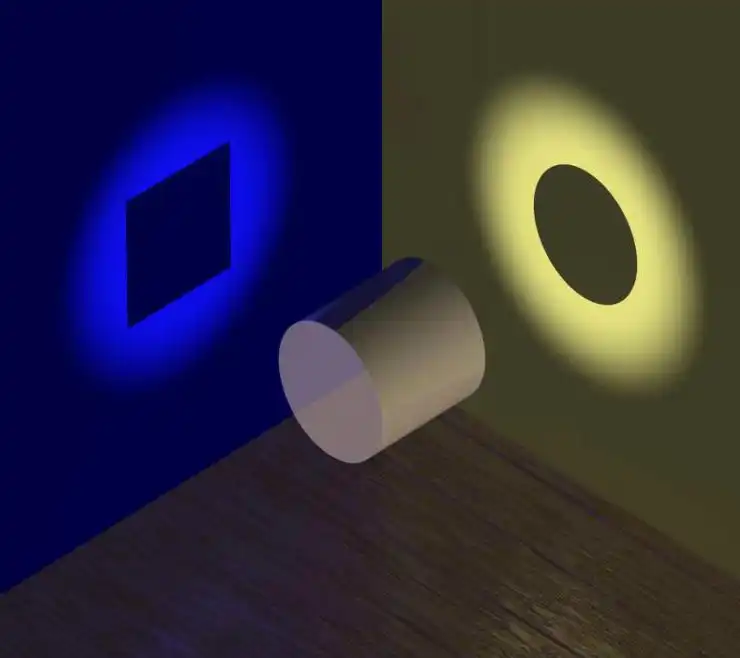
\includegraphics[width=0.4\textwidth]{images/76b33a0418fea16a.png}
\end{center}
\begin{center}
\small\emph{Rappelez-vous cette image d'un objet 3D projeté sur des plans 2D. L'ombre carrée et l'ombre circulaire nous montrent chacune une partie de l'histoire, mais la vraie forme est 3D.}
\end{center}

\begin{keypointbox}
  Il en va de même pour notre jeu de données~! Nos images sont décrites par 3~couleurs différentes (Rouge, Bleu, et Vert).

  Comme les ombres dans cette image, nos deux nuages de points dans l'«~Espace Bleu-vs-Vert~» et l'«~Espace Bleu-vs-Rouge~» ne sont que des \emph{projections} de points 3D sur les plans Z-X et Z-Y.

  Notre «~espace des couleurs~» est tridimensionnel. Les nuages de points ne montrent les données que d'un seul point de vue.
\end{keypointbox}

\begin{activitybox}
  \begin{itemize}
    \item Ouvrez le \href{https://www.desmos.com/3d/qmu6fmrs6h}{nuage de points RVB (Desmos)}.
    \item La table en haut du panneau contient les valeurs Rouge, Vert, et Bleu de notre table \texttt{computed}.
    \item Trouvez le point de l'image \texttt{grass}, qui est tracé comme un point violet.
    \item Le nuage de points pour Bleu-vs-Vert est visible contre la «~paroi arrière~» du cube, chaque image étant un point \textbf{vert}. Comparez-le au nuage de points Pyret sur \emph{Tracer des images}.
    \item Complétez les deux premières sections de \emph{De deux à trois dimensions}.
  \end{itemize}
\end{activitybox}

\img{images/92b411c8c97697a6.png}{width=0.6\textwidth}{Un nuage de points 3D montrant les images sur les axes bleu-vs-rouge-vert, avec les projections de ces points sur les plans bleu-vs-rouge et bleu-vs-vert.}

\begin{keypointbox}
  Nous ne pouvons pas \emph{voir} plus de 3~dimensions à la fois avec nos yeux. Mais l'ordinateur peut calculer la distance dans de nombreuses dimensions. \textbf{Les maths restent vraies}, et nous pouvons utiliser \texttt{distance-similarity}, avec autant d'attributs que nous le voulons.
\end{keypointbox}

\begin{activitybox}
  \textbf{Comment \texttt{distance-similarity} marche-t-elle avec 3~dimensions pour les images avec de l'\textbf{herbe}~?}
  \begin{lstlisting}
distance-similarity(computed, "grass", [list: "red", "green", "blue"])
  \end{lstlisting}

  \begin{itemize}
    \item Essayez-la avec l'ID \texttt{"snow2"}, pour voir comment elle marche avec les images de \textbf{neige}.
    \item Essayez-la avec l'ID \texttt{"red2"}, pour voir comment elle marche avec les images de \textbf{carrés rouges}.
    \item Essayez-la avec l'ID \texttt{"grass\allowbreak-sun"} pour voir comment elle marche avec les images de \textbf{soleil}.
  \end{itemize}

  Essayez d'ajouter d'autres colonnes à votre liste de dimensions. Pouvez-vous identifier un espace de dimension \emph{supérieure} qui marche bien pour les quatre groupes~?
\end{activitybox}

\begin{keypointbox}
  \textbf{Limites de \texttt{distance-similarity}}

  Dans l'ensemble, \texttt{distance-similarity} est une amélioration énorme par rapport à la question «~sont-elles identiques~?~». Mais comme marieur, elle souffre encore de deux problèmes majeurs~:
  \begin{itemize}
    \item \textbf{Elle se concentre sur le \emph{compte} plutôt que sur la \emph{proportion}~:} par exemple, une grande photo de montagne a beaucoup plus de pixels rouges qu'un petit carré rouge — et apparaît donc «~plus proche~» du grand carré rouge que du petit — même si seule une petite fraction de la photo de montagne est rouge.
    \item \textbf{Elle ignore l'\emph{orientation}~:} les humains voient deux images «~majoritairement rouges~» comme similaires, mais la formule de distance ne le fait pas. Elle ne calcule que l'espace entre les points, ignorant où ils se situent \emph{réellement} sur le graphique.
  \end{itemize}
\end{keypointbox}

% ---------- Synthesize ----------
\subsection{Synthèse}

\begin{thinkbox}
  \begin{itemize}
    \item \textbf{Quel rôle chaque colonne joue-t-elle dans la définition de l'espace dans lequel les images sont comparées~?}
    \begin{itemize}
      \item Chaque colonne est associée à un axe.
    \end{itemize}
    \item \textbf{Les nuages de points sont 2D et nos données ont beaucoup plus de dimensions. Les nuages de points nous disent-ils vraiment quelque chose sur nos données~?}
    \begin{itemize}
      \item Oui~! Tout comme nous ne pouvons pas voir une sculpture entière depuis un seul point de vue et que n'importe quel angle nous en dit beaucoup sur la sculpture, les nuages de points manquent d'informations sur d'autres colonnes mais peuvent nous dire beaucoup sur les relations des données dans le plan que nous regardons.
    \end{itemize}
  \end{itemize}
\end{thinkbox}

\newpage

% ===========================================================================
% SECTION 3 : MESURER LES ANGLES DANS L'« ESPACE IMAGE »
% ===========================================================================
\section{Mesurer les angles dans l'«~espace image~»}

\begin{overviewbox}
  Les élèves découvrent la \emph{mesure d'angle} comme notion de similarité. Cela renforce la visualisation des images dans un système spatial.
\end{overviewbox}

% ---------- Launch ----------
\subsection{Lancement~: angle de similarité}

Essayons une autre forme de similarité, qui repose sur l'idée que les images «~à dominante rouge~» se regrouperont toutes sur un axe, et les images «~à dominante bleue~» sur l'autre. La \textbf{similarité d'angle} compare les angles formés par deux rayons tracés depuis deux points jusqu'à l'origine.

\img{images/340821c2f0c96706.png}{width=0.55\textwidth}{Un système de coordonnées 3D avec des points orange représentant le prix vs.\ la qualité des frites vs.\ la qualité des burgers de divers restaurants. Un point vert représente In-N-Out, et des flèches pointent vers lui et le point orange le plus proche. Des lignes sont tracées de ces deux points à l'origine, avec l'angle entre les lignes mesuré à 18~degrés.}

\begin{activitybox}
  Complétez la dernière section de \emph{De deux à trois dimensions}.
\end{activitybox}

\begin{keypointbox}
  Nous pouvons tracer des lignes (appelées «~rayons~») depuis l'origine jusqu'à n'importe quel de nos points-image dans l'espace. Au lieu de calculer la distance entre ces points, nous pouvons calculer \emph{l'angle entre ces lignes}.

  \begin{itemize}
    \item Deux points identiques auront un angle de \textbf{0$^\circ$}, signifiant «~la plus grande similarité possible~».
    \item Deux points qui tombent sur des axes totalement différents (tout-bleu vs.\ tout-rouge, par exemple) auront un angle de \textbf{90$^\circ$}, signifiant «~la moindre similarité possible~».
  \end{itemize}

  Cela résout les deux problèmes de \texttt{distance-similarity}~:
  \begin{itemize}
    \item \textbf{Compte vs.\ proportion~:} l'angle entre nos deux carrés rouges sera de zéro, puisqu'ils tombent tous deux exactement sur l'axe \texttt{red}. Cela identifie correctement que nos deux carrés rouges sont similaires.
    \item \textbf{Orientation~:} la mesure d'angle, par définition, décrit à quel point deux rayons sont orientés de façon proche.
  \end{itemize}
\end{keypointbox}

\begin{thinkbox}
  \begin{itemize}
    \item \textbf{La similarité d'angle fonctionne-t-elle en 1~dimension~? Aurions-nous pu l'utiliser dans notre «~Espace Vert~»~?}
    \begin{itemize}
      \item Non~! Une limite de la similarité d'angle est que l'angle sera \textbf{toujours de zéro} à moins que nous comparions des documents sur plusieurs dimensions.
    \end{itemize}
    \item \textbf{Les images sont-elles les seules choses que nous pouvons tracer dans un espace à 3~dimensions et utiliser la similarité d'angle~?}
    \begin{itemize}
      \item Non~! Nous pourrions tracer n'importe quelles données avec des attributs quantitatifs.
    \end{itemize}
  \end{itemize}
\end{thinkbox}

\begin{activitybox}
  Utilisons notre connaissance des angles pour estimer la similarité d'angle de quelques points dans un espace colorimétrique 2D.

  Complétez \emph{Similarité d'angle (débranché)}.
\end{activitybox}

% ---------- Investigate ----------
\subsection{Exploration~: \texttt{angle-similarity} en Pyret}

Bien sûr, Pyret possède aussi une fonction «~marieur~» pour la similarité d'angle~!

\contrat{\# angle-similarity :: (Table t, String id, List<String> dimensions) -> Table}

\begin{keypointbox}
  Ce marieur fait exactement le même travail que \texttt{distance-similarity}~:
  \begin{itemize}
    \item Nous apportons une image spécifique et lui demandons de trouver une correspondance.
    \item Nous avons des qualités spécifiques qui nous tiennent à cœur.
    \item Le «~marieur~» pense à toutes les images du corpus, et les classe par ordre décroissant de compatibilité. Mais cette fois, il utilise \textbf{l'angle entre les rayons} plutôt que la distance entre les points.
  \end{itemize}
\end{keypointbox}

\begin{activitybox}
  Complétez \emph{Similarité d'angle (Pyret)}.

  \textbf{La mesure des angles est-elle plus proche de la perception humaine que la mesure de distance~?}

  \textbf{Comment \texttt{angle-similarity} marche-t-elle dans notre espace colorimétrique 3D pour les images avec de l'\textbf{herbe}~?}
  \begin{lstlisting}
angle-similarity(computed, "grass", [list: "red", "green", "blue"])
  \end{lstlisting}

  \begin{itemize}
    \item Essayez-la avec l'ID \texttt{"snow2"}, pour voir comment elle marche avec les images de \textbf{neige}.
    \item Essayez-la avec l'ID \texttt{"red2"}, pour voir comment elle marche avec les images de \textbf{carrés rouges}.
    \item Essayez-la avec l'ID \texttt{"grass\allowbreak-sun"} pour voir comment elle marche avec les images de \textbf{soleil}.
    \item Explorez s'il est utile d'ajouter nos colonnes \texttt{WIDTH} et \texttt{HEIGHT}.
  \end{itemize}
\end{activitybox}

\img{images/340821c2f0c96706.png}{width=0.45\textwidth}{Le même système de coordonnées 3D avec les rayons et l'angle entre les points mesuré.}

\begin{keypointbox}
  La similarité d'angle nous a vraiment aidés à améliorer la «~perception~» de la machine sur ce qui rend deux images similaires. À partir d'une image, nous sommes capables de produire de bien meilleurs résultats de recherche~! En repensant à la notion de recherche comme un \textbf{système de recommandation}, vous pourriez aussi imaginer faire la même chose avec d'autres types de données~: par exemple choisir une chanson et demander des recommandations similaires~!
\end{keypointbox}

\begin{instructornotes}
  \textbf{Ce n'est pas juste des maths du collège~?}

  Si~! Les mêmes points et angles que vos élèves tracent et calculent au collège sont au cœur des calculs d'apprentissage automatique qui alimentent tant de choses dans le monde d'aujourd'hui. Même les détecteurs de plagiat qui vérifient peut-être leurs essais calculent des angles. Donc si vos élèves demandent «~quand allons-nous jamais utiliser ça~?~», vous pouvez leur dire «~vous le faites déjà, tout le temps~».

  \vspace{0.3em}
  Si vous avez des élèves plus âgé·es qui ont appris de la trigonométrie, vous voudrez peut-être partager que les vrais systèmes d'apprentissage automatique utilisent le \emph{cosinus} de l'angle. Il y a deux raisons à cela~:
  \begin{itemize}
    \item C'est plus simple de calculer le cosinus directement. (En fait, dans Pyret, \texttt{angle-similarity} calcule d'abord le cosinus, puis convertit le résultat en angle~!)
    \item L'angle lui-même est une valeur quelque peu gênante. L'idée que 0$^\circ$ signifie «~le plus similaire~» et que 90$^\circ$ (l'angle le plus grand) signifie le \emph{moins} de similarité peut être contre-intuitive. En revanche, le cosinus a une plage numérique agréable pour les angles entre 0$^\circ$ et~90$^\circ$, allant de~1 à~0, ce qui le rend pratique dans d'autres contextes mathématiques.
  \end{itemize}

  Pour les besoins de ce programme, vous pouvez ignorer la différence entre similarité d'angle et de cosinus~! Mais pour les élèves qui connaissent le cosinus et sont curieux·ses d'explorer, tous les fichiers de démarrage de notre parcours~IA ont accès à une fonction \texttt{cosine-similarity}.
\end{instructornotes}

\begin{keypointbox}
  \textbf{Limitations par rapport à des outils comme Google Image Search}

  Notre système a encore certaines lacunes comparé à des outils comme Google Image Search~:
  \begin{itemize}
    \item Nous ne pouvons \emph{rechercher que par document}~: nous choisissons une image et trouvons des images similaires.
    \begin{itemize}
      \item Les moteurs de recherche d'images nous permettent de taper un mot comme «~herbe~»~!
      \item Les applications de streaming musical comme Tidal nous permettent de taper un mot comme «~jazz~», plutôt que de nous demander une chanson spécifique.
    \end{itemize}
    \item Nous ne recommandons des correspondances que sur la base d'un seul document~: nous ne pouvons pas trouver des images, des chansons, ou autre chose sur la base d'une \emph{collection} de documents aimés ou non aimés.
  \end{itemize}

  \img{images/35eac0b4625a36db.jpg}{width=0.25\textwidth}{Un robot tenant un livre avec un pouce levé sur la couverture.}

  Certains systèmes d'IA sont capables de reconnaître des parties d'une image («~personne~», «~voiture~», etc.). Cela relève d'une classe d'algorithmes d'IA appelée «~Vision par Ordinateur~», qui s'appuie fortement sur des concepts plus avancés — et plus intensifs en calcul — que nous ne couvrirons pas ici.

  Nous allons utiliser nos cerveaux humains pour voir ces éléments dans nos images, puis explorer si un algorithme piloté par les données peut nous aider à recréer les technologies de recherche d'images, même sans la technologie de Vision par Ordinateur.
\end{keypointbox}

% ---------- Synthesize ----------
\subsection{Synthèse}

\begin{thinkbox}
  \begin{itemize}
    \item \textbf{Il est évident pourquoi \texttt{angle-similarity} fonctionne en deux dimensions~: vous pouvez utiliser un rapporteur sur une feuille de papier au besoin~! Comment pourriez-vous expliquer qu'elle fonctionne encore en \textbf{trois}~dimensions~?}
    \begin{itemize}
      \item Tout ce dont nous avons besoin, c'est de deux rayons partant de l'origine, formant un «~V~» comme les brins d'une fronde. Peu importe comment vous tournez et tordez le «~V~», il définira toujours un plan sur lequel nous pouvons utiliser un rapporteur.
    \end{itemize}
    \item \textbf{Étant donné ce corpus d'images, qui inclut nos carrés rouges, pourquoi ne pouvions-nous pas utiliser la similarité d'angle sur un Espace Bleu-Vert~?}
    \begin{itemize}
      \item La similarité d'angle exige de tracer deux rayons pour que l'angle entre eux puisse être mesuré. Mais nos carrés rouges ont zéro comme valeur pour \texttt{blue} et \texttt{green}, donc leurs coordonnées dans l'Espace Bleu-Vert seraient $(0, 0)$. Il est impossible de tracer une ligne entre un point et lui-même, donc il n'y a aucun moyen de mesurer l'angle entre nos carrés rouges et toute autre image.
    \end{itemize}
    \item \textbf{Y a-t-il des limites à l'utilisation des mesures d'angle pour la similarité, où la distance pourrait être meilleure~?}
    \begin{itemize}
      \item Si nous ne mesurons qu'en 1~dimension, l'angle sera toujours de zéro.
    \end{itemize}
  \end{itemize}
\end{thinkbox}

\newpage

% ===========================================================================
% ANNEXES
% ===========================================================================
\section*{Annexe A~: Trois mesures de similarité}

\begin{center}
\begin{tabularx}{\textwidth}{l X X}
  \toprule
  \textbf{Mesure} & \textbf{Fonction Pyret} & \textbf{Trade-off} \\
  \midrule
  Concordance exacte & «~sont-elles identiques~?~» & Tout ou rien. Trop rigide pour des recommandations. \\
  Distance euclidienne & \texttt{distance-similarity} & Compte la distance entre les points. Ignore la proportion (grande vs.\ petite image) et l'orientation. \\
  Similarité d'angle & \texttt{angle-similarity} & Mesure l'angle entre les rayons depuis l'origine. Capture la proportion et l'orientation, mais nécessite au moins 2~dimensions. \\
  \bottomrule
\end{tabularx}
\end{center}

\section*{Annexe B~: Fichiers du projet}

\begin{center}
\begin{tabularx}{\textwidth}{l X}
  \toprule
  \textbf{Fichier} & \textbf{Description} \\
  \midrule
  \texttt{Images\allowbreak-Similaires\allowbreak-Starter.arr} & Fichier de démarrage Pyret~: charge \texttt{ai-library.arr} depuis Bootstrap, fournit \texttt{distance-similarity}, \texttt{angle-similarity}, \texttt{decorate-image-table}, \texttt{add-bag-cols}, etc. \\
  \texttt{mesurer-similarite.tex} & Document de cours (ce fichier) \\
  \texttt{images/} & 12~images~: captures Google Images, montagnes, papillon, sac de mots, nuages 2D/3D, cylindre, robot \\
  \bottomrule
\end{tabularx}
\end{center}

\vspace{1em}
\textbf{À noter~:} les noms de colonnes (\texttt{ID}, \texttt{DOC}, \texttt{LIKED}, \texttt{DISLIKED}, \texttt{TAGS}, \texttt{LUMINANCE}, \texttt{ENTROPY}, \texttt{SYMMETRY-V}, \dots, \texttt{DOMINANT-RGB-COLORS}, \texttt{red}, \texttt{green}, \texttt{blue}) sont codés en dur dans la bibliothèque \texttt{ai-library.arr} de Bootstrap (1905~lignes) et ne peuvent pas être traduits sans modifier la bibliothèque elle-même. Tous les commentaires du fichier de démarrage sont en français.

\section*{À propos de ces supports}

Ces supports ont été développés en partie grâce au soutien de la \emph{National Science Foundation} (bourses 1042210, 1535276, 1648684, 1738598, 2031479 et 1501927).

\begin{center}
  \textbf{Bootstrap} par la Communauté Bootstrap est sous licence Creative Commons 4.0 Unported.\\
  Cette licence n'accorde pas la permission d'organiser des formations ou du développement professionnel.\\[1em]
  \textit{Traduction et adaptation française réalisées en juillet 2026.}\\
  \textit{Source originale~: \url{https://www.bootstrapworld.org/materials/fall2026/en-us/lessons/measuring-similarity/}}
\end{center}

\end{document}